\documentclass[14pt]{memoir}

\usepackage{geometry}
\usepackage[utf8]{inputenc}
\usepackage{amsmath}
\usepackage{amsfonts}
\usepackage{amssymb}
\usepackage{graphicx}
\usepackage[utf8]{inputenc}
\usepackage{amsmath}
\usepackage{amsfonts}
\usepackage{amssymb}
\usepackage[shortlabels]{enumitem}
\usepackage{listings}
\usepackage{xcolor}
\usepackage[most]{tcolorbox}
\usepackage{mathtools}
\usepackage{float}
\usepackage[colorlinks=false, linktocpage=true]{hyperref}

\usepackage{booktabs}% http://ctan.org/pkg/booktabs
\newcommand{\tabitem}{~~\llap{\textbullet}~~}
\usepackage{longtable}
 
\usepackage{caption}
\DeclareCaptionType{code}[Code Listing][List of Code Listings] 

\definecolor{codegreen}{rgb}{0,0.6,0}
\definecolor{codegray}{rgb}{0.5,0.5,0.5}
\definecolor{codepurple}{rgb}{0.58,0,0.82}
\definecolor{backcolour}{rgb}{0.95,0.95,0.92}
 
\lstdefinestyle{mystyle}{
    backgroundcolor=\color{backcolour},   
    commentstyle=\color{codegreen},
    keywordstyle=\color{magenta},
    numberstyle=\tiny\color{codegray},
    stringstyle=\color{codepurple},
    basicstyle=\ttfamily\footnotesize,
    breakatwhitespace=false,         
    breaklines=true,                 
    captionpos=b,                    
    keepspaces=true,                 
    numbers=left,                    
    numbersep=5pt,                  
    showspaces=false,                
    showstringspaces=false,
    showtabs=false,                  
    tabsize=2
}
 
\lstset{style=mystyle}

\setlength{\parindent}{0em}
\setlength{\parskip}{1em}

\author{Brian Rashap, Ph.D.}
\title{ENGR2910 - Circuit Analysis I}

\geometry{letterpaper, portrait, margin=0.75in}

\begin{document}
\frontmatter

\maketitle


\mainmatter

\chapter{Circuit Variables}

\section{Electrical Engineering: An Overview}

\begin{figure}[h]
\begin{center}
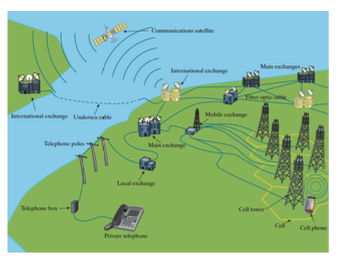
\includegraphics[scale=0.40]{fig/fig01_01.png}
\caption{Telephone System}
\label{fig:01_01}
\end{center}
\end{figure}

Five classifications of electrical systems:
\begin{enumerate}
\item Communication Systems
\item Computer Systems
\item Control Systems
\item Power Systems
\item Signal-Processing Systems
\end{enumerate}

\subsection{Circuit Theory}
Three assumptions:

\section{International System of Units}

\begin{figure}[h]
\begin{center}
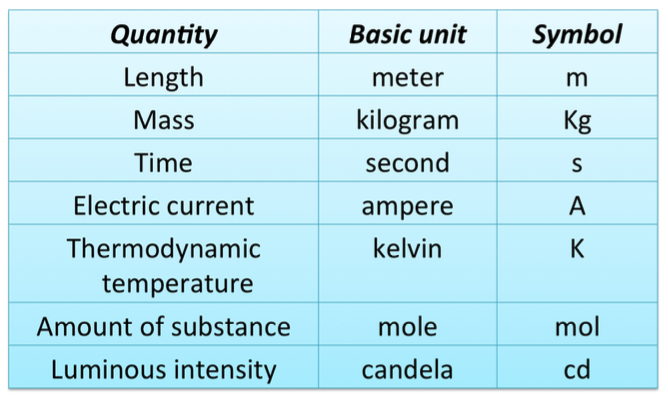
\includegraphics[scale=0.30]{fig/tab01_01.png}
\caption{Scientific Units}
\label{fig:t01_01}
\end{center}
\end{figure}

\begin{figure}[h]
\begin{center}
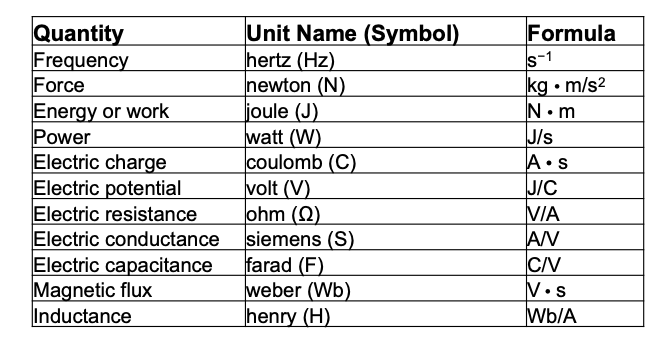
\includegraphics[scale=0.30]{fig/tab01_02.png}
\caption{Derived Units}
\label{fig:t01_02}
\end{center}
\end{figure}

\begin{figure}[h]
\begin{center}
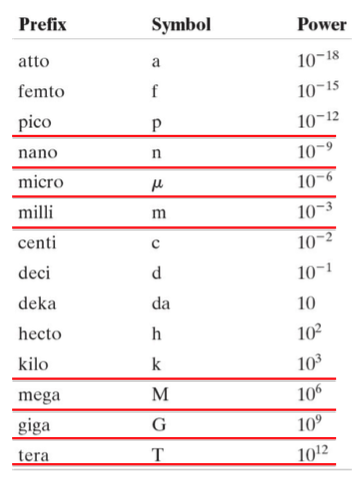
\includegraphics[scale=0.30]{fig/tab01_03.png}
\caption{Powers of 10}
\label{fig:t01_03}
\end{center}
\end{figure}

\subsection{Circuit Analysis: An Overview}

All engineering designs begin with a need that may include a Circuit Model before a physical prototype:

\begin{figure}[h]
\begin{center}
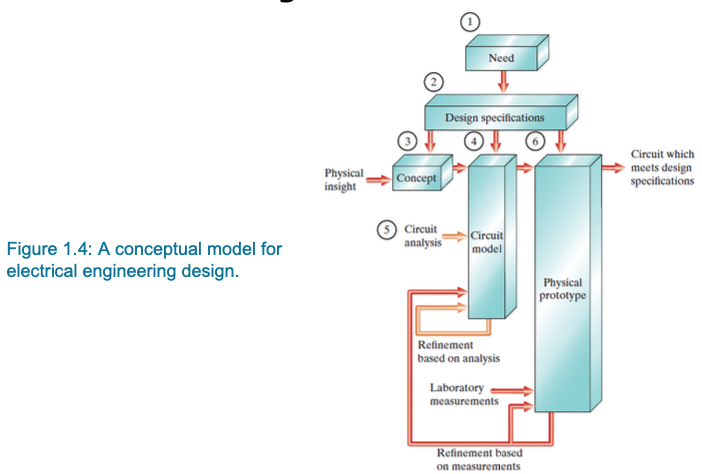
\includegraphics[scale=0.30]{fig/fig01_04.png}
\caption{Conceptual Model for Electrical Engineering Design}
\label{fig:f01_04}
\end{center}
\end{figure}

\subsection{Voltage and Current}

Definition of Voltage ($v$)
\begin{equation}
v = \frac{dw}{dq}
\end{equation}
where w is energy in joules and q is the charge in coulombs. Note that the charge of one electron ($e$ is
\begin{equation}
e = 1.60022 \times 10^{-19} C
\end{equation}

Definition of Current ($i$)
\begin{equation}
i = \frac{dq}{dt},
\end{equation}
where q is charge in coulombs and t is time in seconds.

Note, the direction of current is defined by the direction of flow of positive charge. 

\subsection{DC vs AC}

Direct current is constant with time.
Alternating current varies (sinusoidally) with time and reverses direction

\begin{figure}[h]
\begin{center}
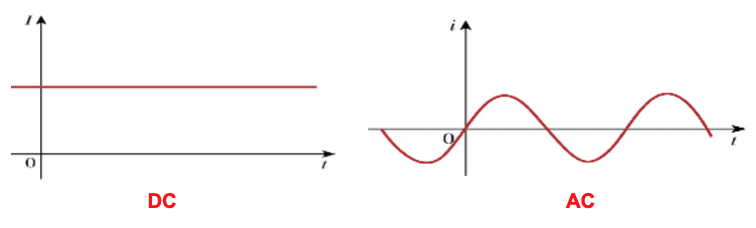
\includegraphics[scale=0.40]{fig/fig01_04a.png}
\caption{DC vs AC}
\label{fig:f01_04a}
\end{center}
\end{figure}

\subsection{Ideal Basic Circuit Element}

The ideal circuit element has three attributes:
\begin{enumerate}
\item It has only two terminals
\item It is described mathematically in terms of current and/or voltage
\item It can not be subdivided to make other elements
\end{enumerate}

\begin{figure}[h]
\begin{center}
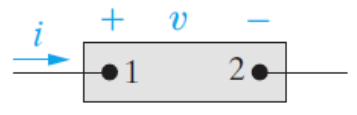
\includegraphics[scale=0.40]{fig/fig01_05.png}
\caption{Ideal basic circuit element}
\label{fig:f01_05}
\end{center}
\end{figure}


\subsubsection{WARNING: Positive Sign Convention}

Whenever the reference direction for the current in an element is in the direction of the reference voltage drop across the element, use a positive sign in any expression that relates he voltage to current. 

\section{Power and Energy}

Power is the energy per unit time

\begin{equation}
p = \frac{dw}{dt},
\end{equation}
where $p$ s power in watts, $w$ is energy in joules, and $t$ is time in seconds. And, where $1W = 1 \frac{J}{s}$.

\begin{equation}
p = \frac{dw}{dt} = (\frac{dw}{dq}) (\frac{dq}{dt})
\end{equation}

therefore,
\begin{equation}
p = v i
\end{equation}

Note, by convention, power is positive ($p>0$) if power is being delivered, and power is negative if power is being extracted from the circuit. 


\subsubsection{Law of Conservation of Energy}

\begin{equation}
\sum p = 0
\end{equation}

Energy is the capacity to do work (measured in J)

\begin{equation}
w = \int_{t_0}^t p dt = \int_{t_0}^t  v i dt
\end{equation}



\begin{figure}[h]
\begin{center}
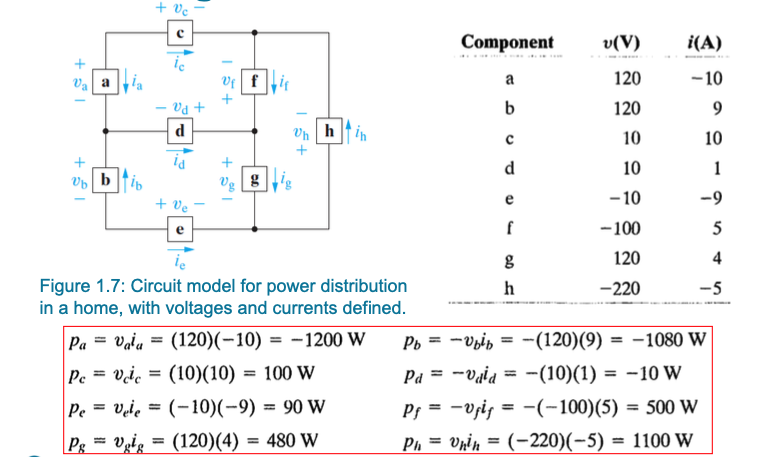
\includegraphics[scale=0.60]{fig/fig01_07a.png}
\caption{Balancing Power Example}
\label{fig:f01_07a}
\end{center}
\end{figure}


\begin{figure}[h]
\begin{center}
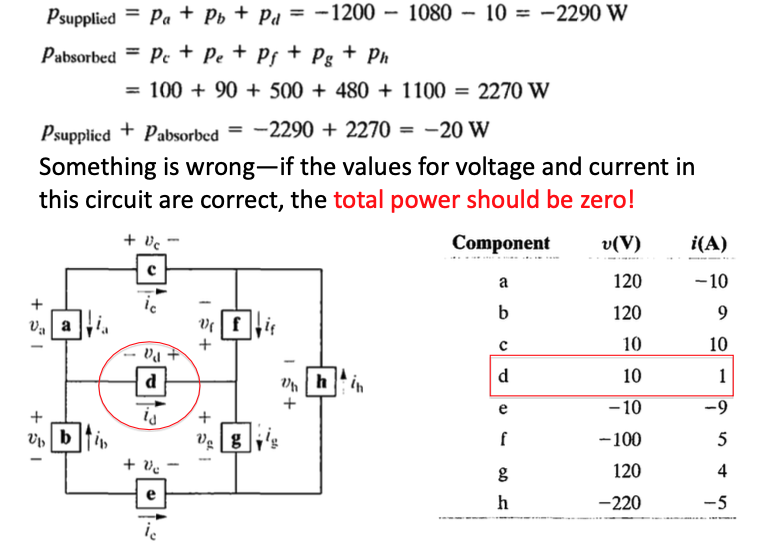
\includegraphics[scale=0.60]{fig/fig01_07b.png}
\caption{Balancing Power Correction}
\label{fig:f01_07b}
\end{center}
\end{figure}

\chapter{Circuit Elements}

\section{Voltage and Current Sources}


When we speak of circuit elements, it is important to differentiate between the physical device itself and the mathematical model which we will use to analyze its behavior in a circuit. We will use the expression circuit element to refer to the mathematical model. All the simple circuit elements that we will consider can be classified according to the relationship between current through the element to the voltage across the element.

\begin{figure}[h]
\begin{center}
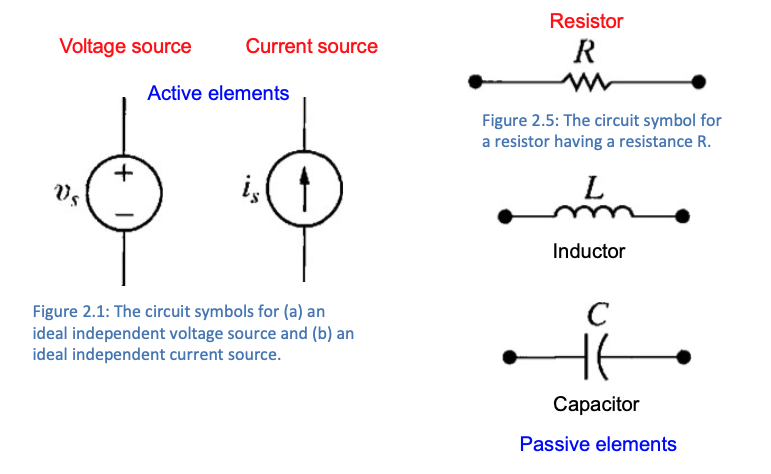
\includegraphics[scale=0.60]{fig/fig02_01.png}
\caption{Five Basic Circuit Elements}
\label{fig:f02_01}
\end{center}
\end{figure}

A dependent source establishes a voltage or current whose value depends on the value of a voltage or current elsewhere in the circuit. You cannot specify the value of a dependent source unless you know the value of the voltage or current on which it depends.

There are four kinds of controlled sources:
\begin{itemize}
\item current-controlled current source (CCCS)
\item voltage-controlled current source (VCCS)
\item voltage-controlled voltage source, (VCVS)
\item current-controlled voltage source, (CCVS)
\end{itemize}

\begin{figure}[h]
\begin{center}
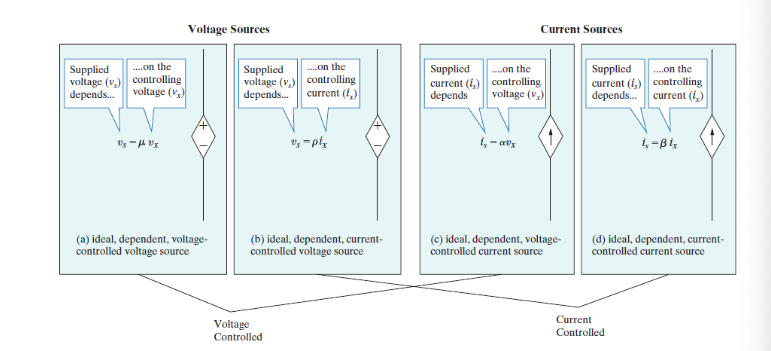
\includegraphics[scale=0.60]{fig/fig02_02.png}
\caption{Four Controlled Sources}
\label{fig:f02_02}
\end{center}
\end{figure}

\section{Electrical Resistance (Ohm's Law)}
Resistance is the capacity of materials to impede the flow of current or, more specifically, the flow of electric charge. The circuit element used to model this behavior is the resistor. The linear resistor is the simplest passive element.

\subsection{Ohm's Law}
The relationship between Voltage and Current was empirically determined by Goerg Ohm\footnote{A presented in a paper published in 1827}

\begin{figure}[H]
\begin{center}
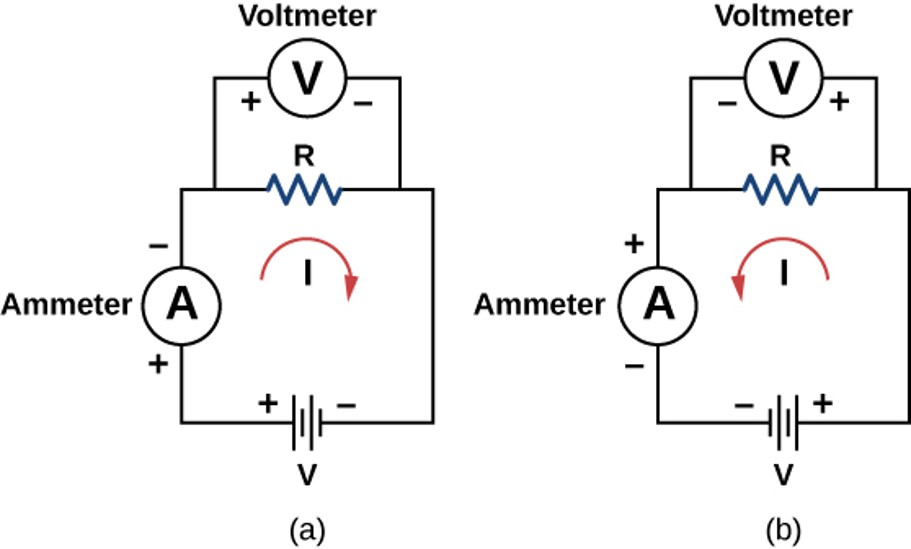
\includegraphics[scale=0.50]{fig/fig_09_19.jpg}
\caption{Goerg Ohm's Setup}
\label{fig:09_19}
\end{center}
\end{figure}

\begin{figure}[H]
\begin{center}
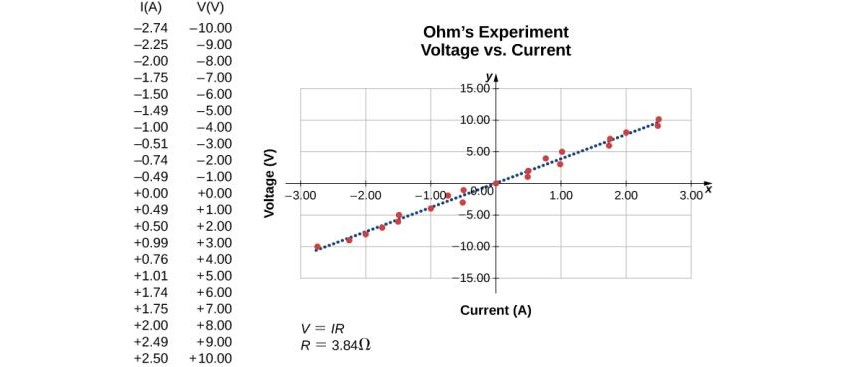
\includegraphics[scale=0.50]{fig/fig_09_20.jpg}
\caption{Goerg Ohm's Data}
\label{fig:09_20}
\end{center}
\end{figure}

Ohm's Law
\begin{equation}
V = I \cdot R
\end{equation}


\section{Kirchhoff's Laws}

\subsection{Kirchhoff's First Law (the Node Law or the Junction Rule)} 
The sum of all currents entering a junction must equal the sum of all currents leaving the junction.

\begin{figure}[H]
\begin{center}
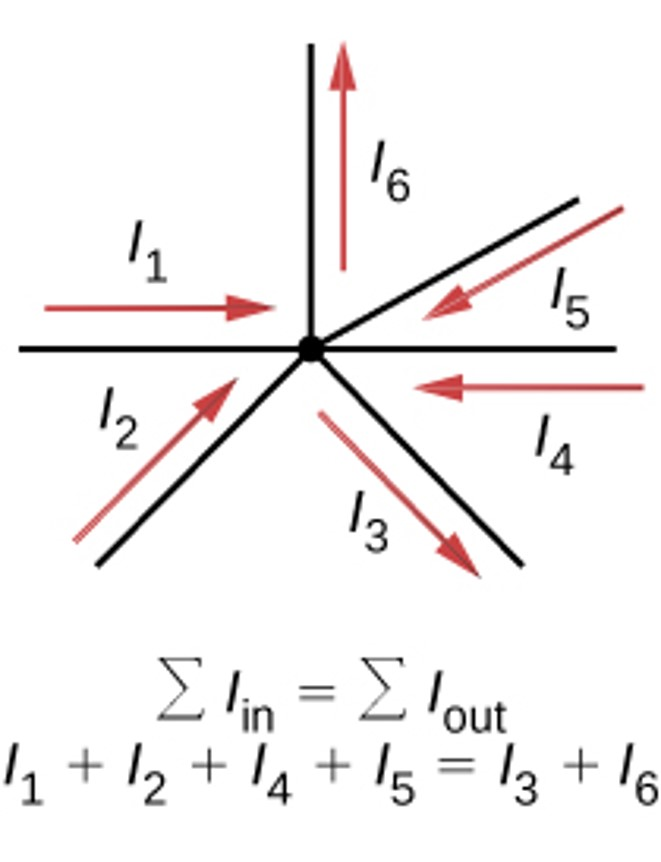
\includegraphics[scale=0.50]{fig/fig_10_20.jpg}
\caption{Kirchholff's Node Law}
\label{fig:10_20}
\end{center}
\end{figure}

\begin{equation}
\sum I_{in} = \sum I_{out}
\end{equation}

\begin{figure}[H]
\begin{center}
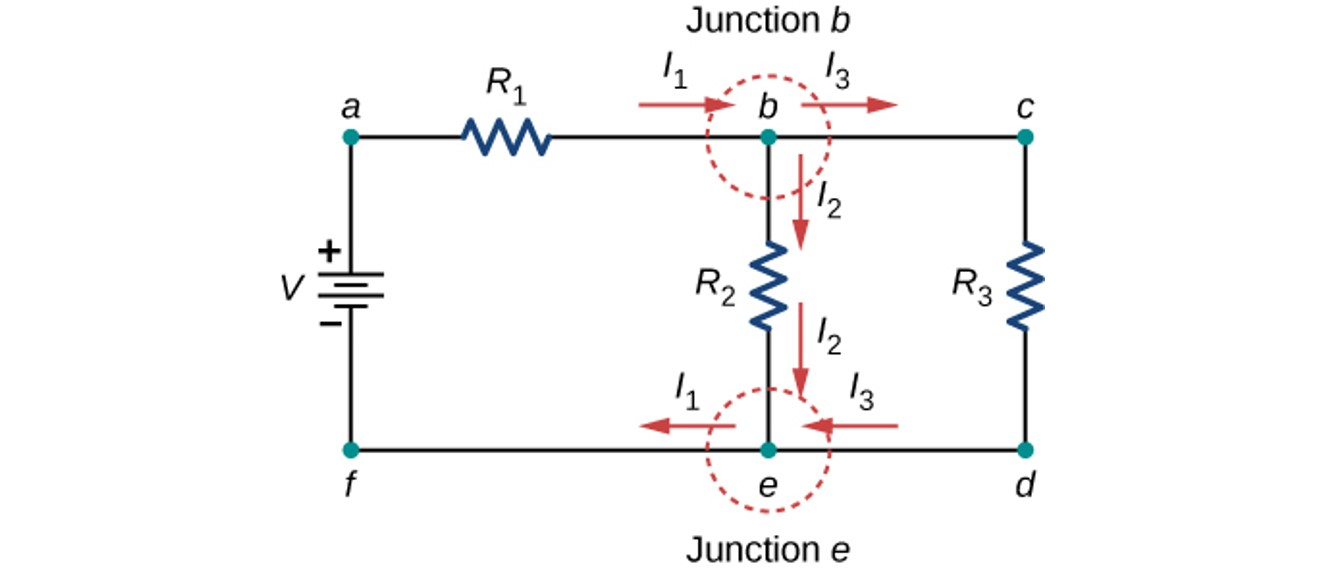
\includegraphics[scale=0.50]{fig/fig_10_24.jpg}
\caption{Kirchholff's Node Law Example}
\label{fig:10_24}
\end{center}
\end{figure}

\subsection{Kirchhoff's Second Law (the Loop Law or the Loop Rule)}

The sum off all potential differences, including those supplied by voltage sources and resistive elements, around a closed loop equals zero.

\begin{figure}[H]
\begin{center}
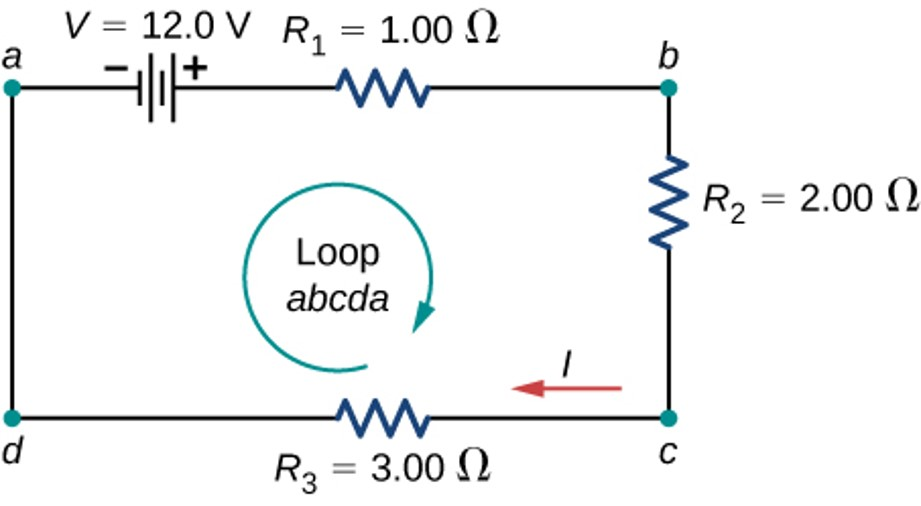
\includegraphics[scale=0.50]{fig/fig_10_21.jpg}
\caption{Kirchholff's Loop Law}
\label{fig:10_21}
\end{center}
\end{figure}

\begin{equation}
\sum_{closed loop} V = 0
\end{equation}

\begin{figure}[H]
\begin{center}
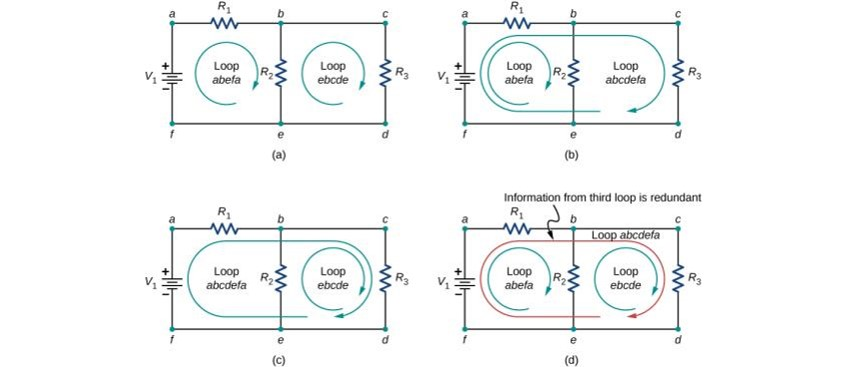
\includegraphics[scale=0.50]{fig/fig_10_25.jpg}
\caption{Kirchholff's Loop Law Example}
\label{fig:10_25}
\end{center}
\end{figure}

\section{Kirchhoff Examples}

\begin{figure}[H]
\begin{center}
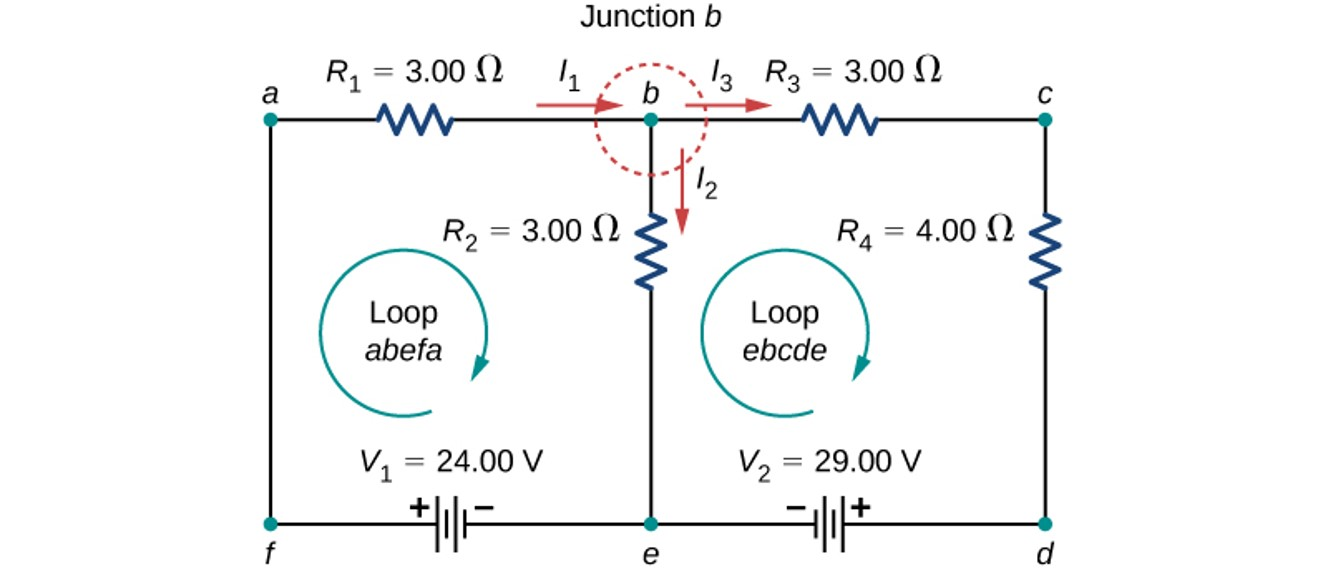
\includegraphics[scale=0.50]{fig/fig_10_28.jpg}
\caption{Kirchholff Example}
\label{fig:10_28}
\end{center}
\end{figure}

\begin{figure}[H]
\begin{center}
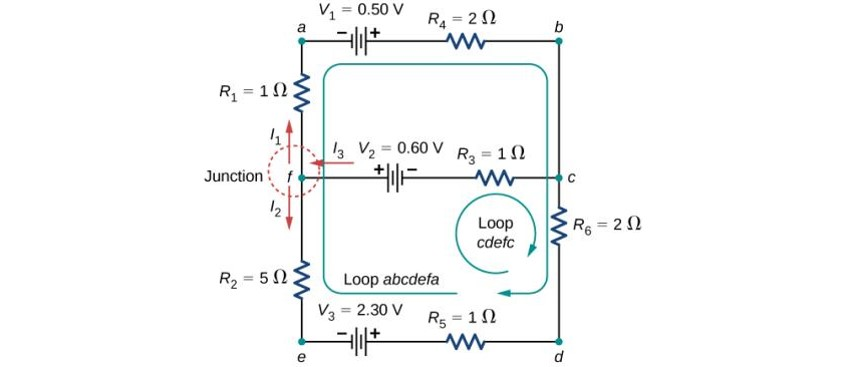
\includegraphics[scale=0.50]{fig/fig_10_29.jpg}
\caption{Kirchholff Examples}
\label{fig:10_29}
\end{center}
\end{figure}

\section{Circuits Containing Dependent Sources}

\begin{figure}[H]
\begin{center}
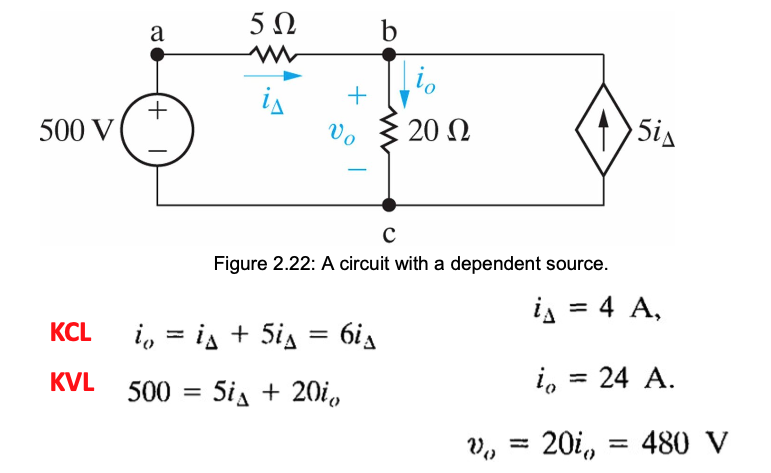
\includegraphics[scale=0.50]{fig/fig02_22.png}
\caption{Controlled Sources}
\label{fig:fig02_22}
\end{center}
\end{figure}


\chapter{Simple Resistive Circuits}

\section{Resistors in Series}

\begin{figure}[H]
\begin{center}
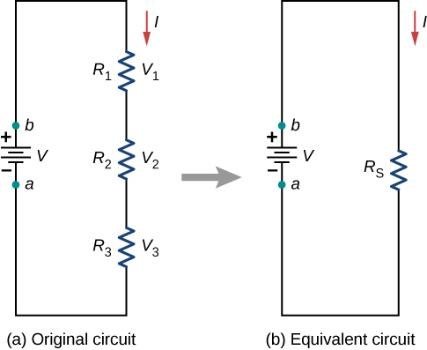
\includegraphics[scale=0.50]{fig/fig_10_12.jpg}
\caption{Resistors in Series}
\label{fig:10_12}
\end{center}
\end{figure}

For resistors in Series

\begin{equation}
V = V_1 + V_2 + V_3
\end{equation}

\begin{equation}
V = 1R_1 + 1R_2 + 1R_3
\end{equation}

\begin{equation}
I = \frac{V}{R_1 + R_2 + R_3}
\end{equation}

So

\begin{equation}
R_{eq} = \sum_{i=1}^{N} R_i
\end{equation}

\begin{figure}[H]
\begin{center}
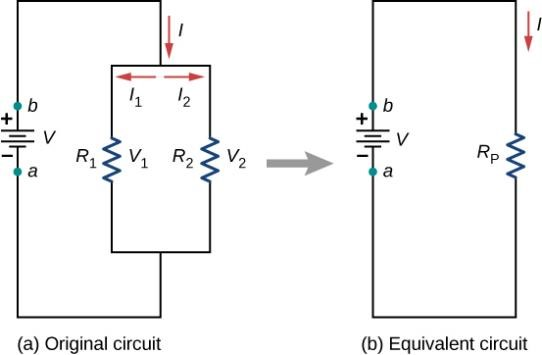
\includegraphics[scale=0.50]{fig/fig_10_14.jpg}
\caption{Resistors Parallel}
\label{fig:10_14}
\end{center}
\end{figure}

\section{Resistors in Parallel}

\begin{equation}
V = V_1 = V_2
\end{equation}

\begin{equation}
I = I_1 + I_2
\end{equation}

\begin{equation}
\frac{V}{R_{eq}} = \frac{V_1}{R_1} + \frac{V_2}{R_2}
\end{equation}

Because the Voltage is equal across the resistors
\begin{equation}
\frac{1}{R_{eq}} = \frac{1}{R_1} + \frac{1}{R_2}
\end{equation}

Or, more generically

\begin{equation}
R_{eq} = (\sum_{i=1}{N} \frac{1}{R_i})^{-1}
\end{equation}



\begin{figure}[H]
\begin{center}
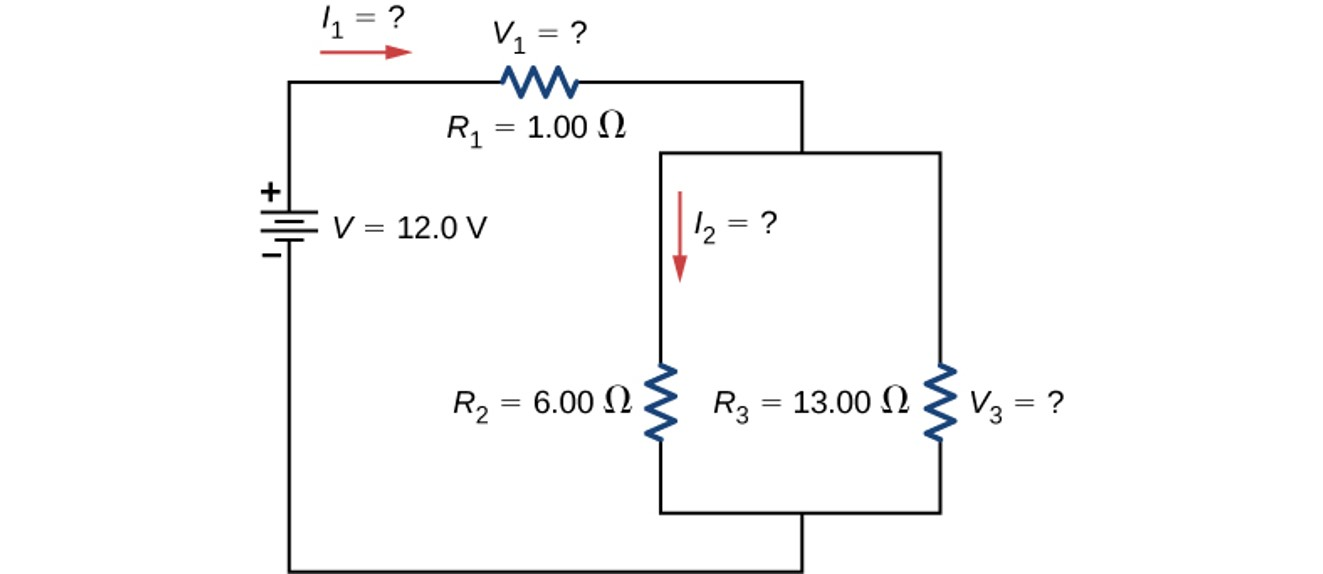
\includegraphics[scale=0.50]{fig/fig_10_16.jpg}
\caption{Resistors in Series and Parallel}
\label{fig:10_16}
\end{center}
\end{figure}


\section{Divider Circuits}

\begin{figure}[H]
\begin{center}
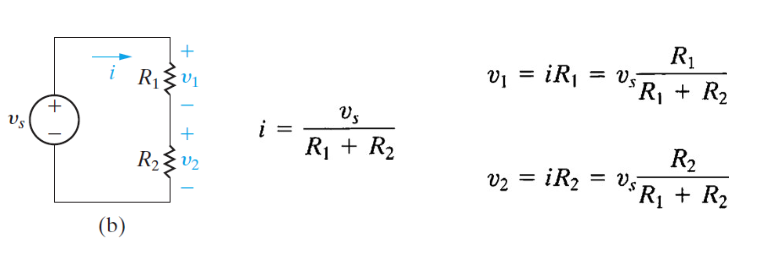
\includegraphics[scale=0.50]{fig/fig03_14.png}
\caption{Voltage Divider}
\label{fig:fig03_14}
\end{center}
\end{figure}


\begin{figure}[H]
\begin{center}
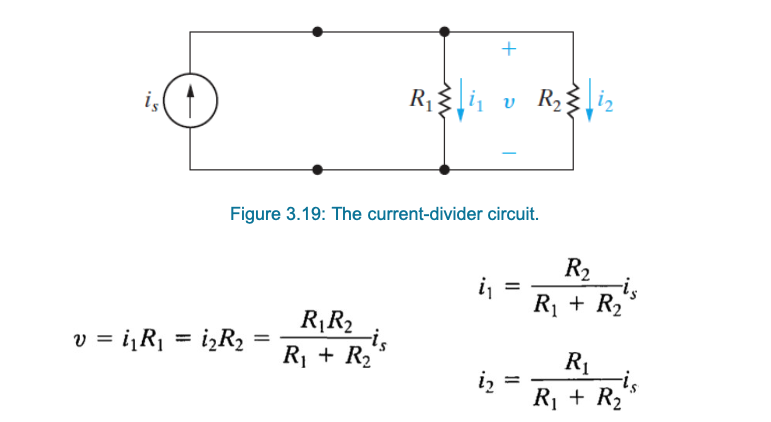
\includegraphics[scale=0.50]{fig/fig03_19.png}
\caption{Current Divider}
\label{fig:fig03_19}
\end{center}
\end{figure}

\subsection{With a Load}

\begin{figure}[H]
\begin{center}
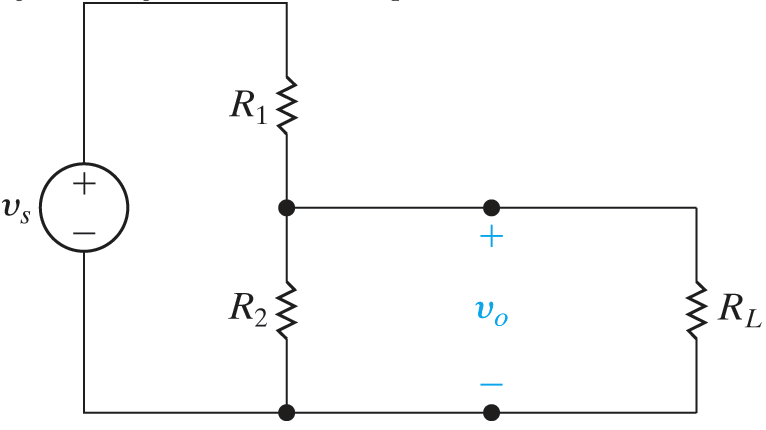
\includegraphics[scale=0.50]{fig/fig03_17.png}
\caption{Voltage Divider with Load}
\label{fig:fig03_17}
\end{center}
\end{figure}

\begin{equation}
v_0 = \frac{R_{eq}}{R_1+R_{eq}} v_s
\end{equation}

where

\begin{equation}
R_{eq} = \frac{R_2 R_L}{R_2 + R_L}
\end{equation}

substituting 

\begin{equation}
v_0 = \frac{R_2}{R_1 [1 + \frac{R_2}{R_L}] + R_2} v_s
\end{equation}

\section{Measuring Voltage and Current}

\begin{itemize}
\item An ammeter is an instrument designed to measure current; it is placed in series with the circuit element whose current is being measured. 
\item A voltmeter is an instrument designed to measure voltage; it is placed in parallel with the circuit element whose current is being measured. 
\end{itemize}

\begin{figure}[H]
\begin{center}
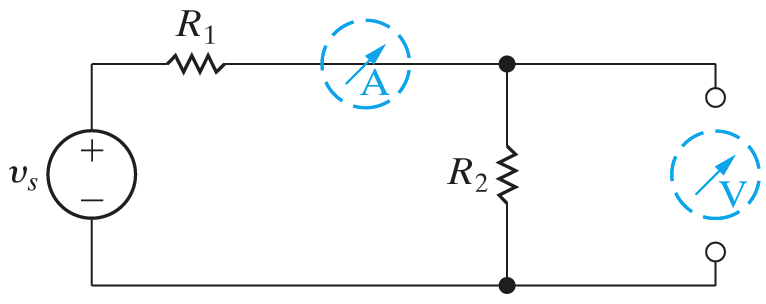
\includegraphics[scale=0.50]{fig/fig03_24.png}
\caption{Short-circuit model for ideal ammeter, and open-circuit model for ideal volt meter}
\label{fig:fig03_24}
\end{center}
\end{figure}

\subsection{d'Arsonval meter}

\begin{figure}[H]
\begin{center}
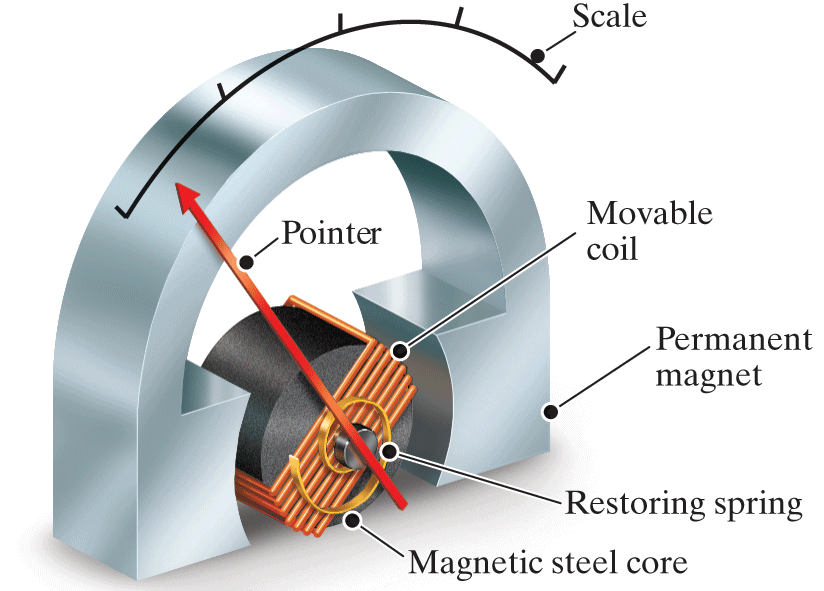
\includegraphics[scale=0.50]{fig/fig03_25.png}
\caption{d'Arsonval meter movement}
\label{fig:fig03_25}
\end{center}
\end{figure}

\subsection{Non-ideal meters}

\begin{figure}[H]
\begin{center}
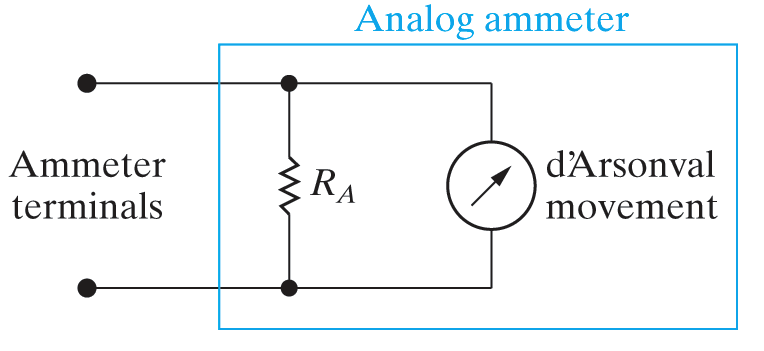
\includegraphics[scale=0.50]{fig/fig03_26.png}
\caption{Non-Ideal Ammeter}
\label{fig:fig03_26}
\end{center}
\end{figure}

\begin{figure}[H]
\begin{center}
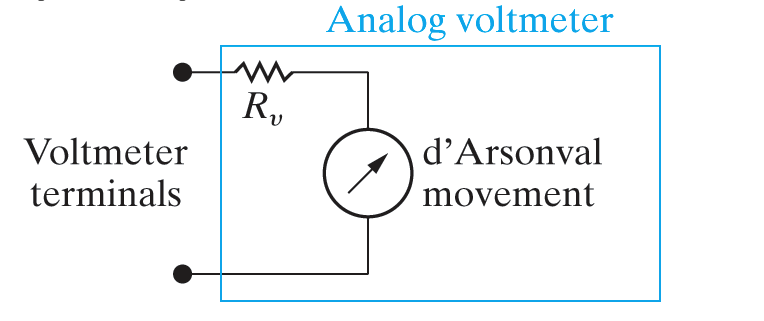
\includegraphics[scale=0.50]{fig/fig03_27.png}
\caption{Non-ideal Voltmeter}
\label{fig:fig03_27}
\end{center}
\end{figure}



\appendix

\chapter{Integration by Trig Substitution}
\label{sec:trigsub}

Find the integral of 

\begin{equation}
\int \frac{1}{(a^2 + x^2)^{\frac{3}{2}}}
\end{equation}

Integrate by trig substitution by setting $x = a\tan{u}$ which leads to 

\begin{equation}
\frac{dx}{du} = \frac{a \tan{u}}{du} = \frac{a}{\cos^2{u}}
\end{equation}

Which leads to 
\begin{equation}
dx = ( \frac{a}{\cos^2{u}}) du 
\end{equation}

Thus

\begin{equation}
\int \frac{1}{(a^2 + x^2)^{\frac{3}{2}}} =  \int \frac{1}{(a^2 + (a\tan{(u)})^2)^{\frac{3}{2}}} ( \frac{a}{\cos^2{(u)}}) du
\end{equation}

\begin{equation}
=  \int \frac{1}{(a^2)^{\frac{3}{2}} (1 + \tan^2{(u)})^{\frac{3}{2}}} ( \frac{a}{\cos^2{(u)}}) du
\end{equation}

\begin{equation}
=  \int \frac{1}{(a^3)(\frac{1}{\cos^2(u)})^{\frac{3}{2}}} ( \frac{a}{\cos^2{(u)}}) du
\end{equation}

\begin{equation}
=  \frac{1}{a^2} \int \frac{1}{(\frac{1}{\cos^2(u)})^{\frac{3}{2}}} ( \frac{1}{\cos^2{(u)}}) du
\end{equation}

\begin{equation}
=  \frac{1}{a^2} \int \frac{1}{(\frac{1}{\cos^3(u)})} ( \frac{1}{\cos^2{(u)}}) du
\end{equation}

\begin{equation}
=  \frac{1}{a^2} \int \cos{(u)} du
\end{equation}

\begin{equation}
=  \frac{1}{a^2} \sin{(u)} + C
\end{equation}


From the above $\arctan{(\frac{x}{a})} = u$ so

\begin{equation}
=  \frac{1}{a^2} \sin{(\arctan{(\frac{x}{a})})} + C
\end{equation}

\begin{equation}
=  \frac{1}{a^2} [\frac{\frac{x}{a}}{\sqrt{1+(\frac{x}{a})^2}}] + C
\end{equation}

\begin{equation}
=  \frac{x}{a^3} [\frac{1}{\frac{1}{a} \sqrt{a^2+x^2}}] + C
\end{equation}

Which finally leads to

\begin{equation}
\int \frac{1}{(a^2 + x^2)^{\frac{3}{2}}} =  \frac{x}{a^2} [\frac{1}{\sqrt{a^2+x^2}}] + C
\end{equation}





\chapter{Chain Rule}

\begin{equation}
\frac{d}{dx} (\frac{1}{\sqrt{x^2+R^2}}) = \frac{d}{dx} (x^2+R^2)^{-\frac{1}{2}} 
\end{equation}

The chain rule $ f(g(x))' = f'(g(x) \cdot g'(x)$. In this case $g(x) = x^2 + R^2$. From this

\begin{equation}
f(g(x)) = g(x)^{-\frac{1}{2}} 
\end{equation}

thus  

\begin{equation}
f'(g(x)) = -\frac{1}{2} g(x)^{-\frac{3}{2}} 
\end{equation}

and

\begin{equation}
g'(x) = 2x
\end{equation}

Thus

\begin{equation}
f(g(x))' =  -\frac{1}{2} g(x)^{-\frac{3}{2}}  \cdot 2x
\end{equation}

\begin{equation}
\frac{d}{dx} (\frac{1}{\sqrt{x^2+R^2}}) = \frac{-x}{(x^2 + R^2)^\frac{3}{2}}
\end{equation}


\end{document}
